\documentclass[a4paper,10pt]{article}
\usepackage{color}
\usepackage[utf8]{inputenc}


%Packages
\usepackage{graphicx}
\usepackage{grffile}
\usepackage{float}


\title{Testing Document for PowerCloud}

\author{Marc Antel, 12026973\\ Brandon Wardley, 29005150\\ Stuart Andrews, 12153983\\ Mothusi Masibi, 12004589}
\date{\today}

\begin{document}
	\maketitle
	\newpage
	\section{Test Plan}
		\subsection{Firmware}
			We're using Manual Testing to test the firmware due to the fact that the firmware has to be compiled using the Particle Cloud.
			
			However, in due course, we intend to find a workaround in order to test the firmware using a testing framework.
			
			The following features of the firmware are tested:
			\begin{itemize}
				\item Store to EEPROM using a struct.
				\item Store to EEPROM using raw values.
				\item Retrieve from EEPROM.
				\item Check EEPROM for data.
				\item MQTT connect, which establishes a reliable connection to the server.
				\item MQTT publish, which publishes JSON to the server.
			\end{itemize}
			
		\subsection{Application Server}
			We're using \textbf{JUnit} to test the major features of our application server.
			Detailed descriptions of these features are as follows:
				\begin{itemize}
					\item Concurrent MQTT Client Connections.
					\item Validate Data from Client.
					\item Store data to Firebase.
				\end{itemize}
				
	\section{Test Design}
	The tests were implemented as follows for each of the components of the entire system.
	\subsection{Test Procedure Description}
		\subsubsection{Firmware}
		\textbf{Store to EEPROM using a struct.}
			\begin{enumerate}
				\item Create the appropriate structure.
				\item Attempt to store said structure.
				\item Create an empty struct.
				\item Attempt to store an empty struct.
				\item Retrieve structs from EEPROM and verify that they are correct.
			\end{enumerate}
		\textbf{Store to EEPROM using raw values.}
			\begin{enumerate}
				\item Declare raw values which need to be stored.
				\item Attempt to store these accpetable values.
				\item Retrieve data from EEPROM and verify that it is correct. 
			\end{enumerate}
		\textbf{Retrieve from EEPROM.}
			\begin{enumerate}
				\item Create multiple struct objects.
				\item Store these struct objects to EEPROM.
				\item Attempt to retreive stored objects.
				\item Verify that the objects are correct.
				\item Clear Memory.
				\item Attempt to retrieve objects again.
			\end{enumerate}
			
		\textbf{Check EEPROM for data.}
			\begin{enumerate}
				\item Calculate how many struct objects can be stored in EEPROM.
				\item Create enough struct objects to fill EEPROM to capacity.
				\item Call appropriate function to determine if the EEPROM is full.
				\item Create half the capacity of struct objects.
				\item Store these struct objects to EEPROM.
				\item Call appropriate function to determine if the EEPROM is full.
			\end{enumerate}
		\textbf{MQTT connect, which establishes a reliable connection to the server.}
			\begin{enumerate}
				\item Provide incorrect host IP.
				\item Attempt to connect.
				\item Proivde correct host IP.
				\item Attempt to connect.
			\end{enumerate}
		\textbf{MQTT publish, which publishes JSON to the server.}
			\begin{enumerate}
				\item Ensure connection to server is established.
				\item Publish well-formed JSON.
				\item Publish malformed JSON.
				\item Ensure ACK packets are received on both occasions.
			\end{enumerate}
			
		\subsubsection{Application Server}
		
		\textbf{Concurrent MQTT Client Connections.}
		\begin{enumerate}
			\item Connect to server using Particle Photon.
			\item Connect to server using MQTT Lens plugin.
			\item Publish messages to server from photon and plugin concurrently.
			\item Evaluate Firebase to ensure data is stored correctly.
		\end{enumerate}
		\textbf{Validate Data from Client.}
		\begin{enumerate}
			\item Once a message has been received from a client.
			\item Extract payload from message.
			\item Parse JSON String into JSON object.
			\item Catch exception if necessary.
			\item Ensure JSON Object is accessible.
		\end{enumerate}
		\textbf{Store data to Firebase.}
		\begin{enumerate}
			\item Receive a continuous stream of messages from MQTT Clients.
			\item Attempt to store all messages to firebase.
			\item Verify that all messages are present.
			\item Receive a continuous stream of messages with a 10 second delay.
			\item Attempt to store messages to Firebase.
			\item Verify that all messages are present.
		\end{enumerate}
			
	\section{Test Execution}
		\subsection{Test Incident Report}
			\subsubsection{Firmware}
			The following incidents occured during firmware testing. Namely during:
			\textbf{Testing the connect and publish:}
				\begin{enumerate}
					\item Particle Photon disconnects from WIFI after concurrent publish events.
					\item Particle Photon does not continue publishing after disconnecting.
				\end{enumerate}
			\textbf{Testing the EEPROM}
			No incidents occured with regards to testing the EEPROM.
			\subsubsection{Application Server}
			The following incidents occured during application server testing. Namely during:
			\textbf{Storing to Firebase}
				\begin{enumerate}
					\item When receiving continous messages from clients, some messages are not stored to Firebase.
				\end{enumerate}
			
		\subsection{Test Log}
			\subsubsection{Application Server}
					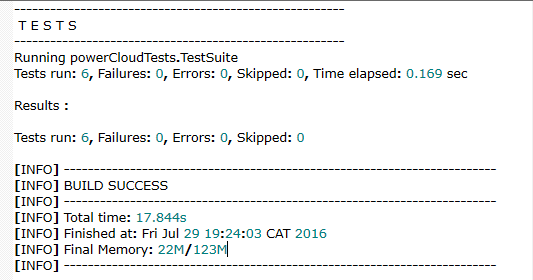
\includegraphics[width=\textwidth]{images/TestOutput.png}
	
	\section{Test Summary Report}
		\subsection{Firmware}
			The current state of the Firmware is as follows.
			\\The following tests need to be implemented and assessed:
			\begin{itemize}
				\item Attempt to publish a message without establishing a reliable connection to the server.
				\item Attempt to overflow variables.
				\item Attempt store incorrect datatypes.
				\item Test if EEPROM clears once full.
				\item Check data persists after device loses power.
				\item Criteria which would cause the device to disconnect or reboot.
			\end{itemize}
		\subsection{Application Server}
		The current state of the Application Server is as follows.
		\\The following tests need to be implemented and assessed:
			\begin{itemize}
				\item Test whether messages received from clients contain the correct data.
				\item Attempt to store malformed JSON to Firebase.
				\item Test store methods using parameterized test.
				\item Test \textit{checkMonth()} with parameterized tests.
				\item Test \textit{validateID()} using parameterized tests.
				\item Test appropriate exceptions which are included within the exceptions package.
			\end{itemize}
			
		As a whole, the system functions as expected using expected parameters.
		The next round of testing will be to ensure that the system functions correctly under unexpected conditions.
\end{document}